\documentclass{standalone}
\usepackage{tikz}
\begin{document}
			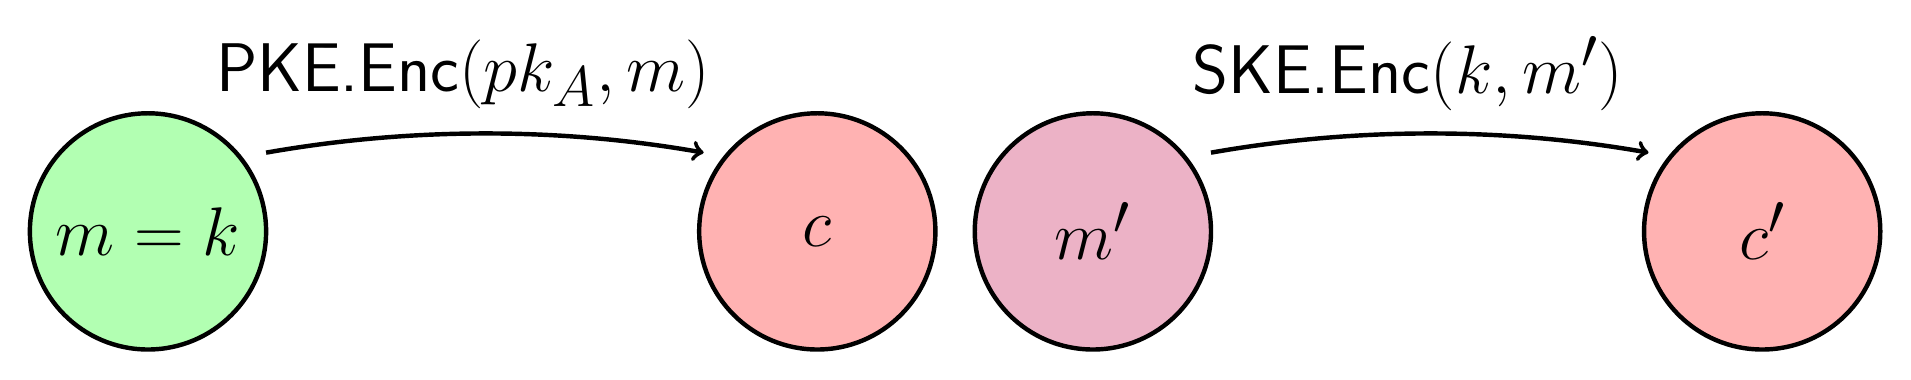
\begin{tikzpicture}
				\draw[ultra thick, fill=green!30] (0,0) circle (1.5);
				\draw[ultra thick, fill=red!30] (8.5,0) circle (1.5);
				\draw[ultra thick, ->] (1.5,1) arc (100:80:16);
				
				\node[] (x) at (0,0) {\Huge $m=k$};
				\node[] (e) at (4,2) {\Huge {\textsf{PKE.Enc}$(pk_A,m)$}};
				\node[] (fx) at (8.5,0) {\Huge $c$};
				
				\draw[ultra thick, fill=purple!30] (12,0) circle (1.5);
				\draw[ultra thick, fill=red!30] (20.5,0) circle (1.5);
				\draw[ultra thick, ->] (13.5,1) arc (100:80:16);
				\node[] (x) at (12,0) {\Huge $m'$};
				\node[] (e) at (16,2) {\Huge {\textsf{SKE.Enc}$(k,m')$}};
				\node[] (fx) at (20.5,0) {\Huge $c'$};
			\end{tikzpicture}
\end{document}
